%%% Local Variables:
%%% mode: latex
%%% TeX-master: t
%%% End:

%\documentclass[doctor,secret]{ucasthesis}
\documentclass[master, secret]{ucasthesis}
%\documentclass[doctor]{ucasthesis}
% \documentclass[%
%   master|doctor, % mandatory option
%   secret,
%   arialtoc,arialtitle]{ucasthesis}

% 所有其他可能用到的包都统一放到这里了,可以根据自己的实际添加或者删除。
\usepackage{ucastils}

\usepackage{booktabs}% http://ctan.org/pkg/booktabs
\newcommand{\tabitem}{~~\llap{\textbullet}~~}


\usepackage{supertabular} %跨页表格
\usepackage{colortbl} %彩色表格宏包
\usepackage{tablefootnote}

\usepackage{longtable}
\usepackage{array} % for extrarowheight
\setlength{\extrarowheight}{1.5pt}

%伪代码
\usepackage{algorithm}
\usepackage{algorithmicx}
\usepackage{algpseudocode}
\usepackage{amsmath}

\floatname{algorithm}{算法}
\renewcommand{\algorithmicrequire}{\textbf{输入:}}
\renewcommand{\algorithmicensure}{\textbf{输出:}}

% 你可以在这里修改配置文件中的定义,导言区可以使用中文。
% \def\myname{胡庆海}

\begin{document}

% 定义所有的eps文件在 figures 子目录下
\graphicspath{{figures/}}

%%% 封面部分
\frontmatter

%%% Local Variables:
%%% mode: latex
%%% TeX-master: t
%%% End:
\secretcontent{绝密}

\ctitle{龙芯3A下Mesa3D图形库的性能优化}
% 根据自己的情况选,不用这样复杂
\makeatletter

\makeatother

\cdegree{工程硕士}
\cdepartment[计算所]{中国科学院计算技术研究所}
\cmajor{计算机技术}
\cauthor{胡庆海} 
\csupervisor{胡伟武\hspace{1em}研究员}
\csupervisorplace{中国科学院计算技术研究所}
% 如果没有副指导老师或者联合指导老师,把下面两行相应的删除即可。


% 日期自动生成,如果你要自己写就改这个cdate
%\cdate{\CJKdigits{\the\year}年\CJKnumber{\the\month}月}

% 博士后部分
% \cfirstdiscipline{计算机科学与技术}
% \cseconddiscipline{系统结构}
% \postdoctordate{2009年7月——2011年7月}

\etitle{Performance Optimization of Mesa3D Graphics Library on Loongson 3A Platform}
% 这块比较复杂,需要分情况讨论:
% 1. 学术型硕士
%    \edegree:必须为Master of Arts或Master of Science(注意大小写)
%              “哲学、文学、历史学、法学、教育学、艺术学门类,公共管理学科
%               填写Master of Arts,其它填写Master of Science”
%    \emajor:“获得一级学科授权的学科填写一级学科名称,其它填写二级学科名称”
% 2. 学术型博士
%    \edegree:Doctor of Philosophy(注意大小写)
%    \emajor:“获得一级学科授权的学科填写一级学科名称,其它填写二级学科名称”

\edegree{Master of Computer Architecture}
\eauthor{Hu Qinghai}
\edepartment{Institute of Computing Technology\\Chinese Academy of Sciences}
\emajor{Computer Technology}
\esupervisor{Hu Weiwu}

% 这个日期也会自动生成,你要改么?
% \edate{December, 2005}

% 定义中英文摘要和关键字
\begin{cabstract}

  OpenGL是行业领域中最为广泛接纳的2D/3D图形API, 其自诞生至今已催生了各种计算机平台及设备上的数千优秀应用程序。而随着龙芯CPU的产业化加速,基于OpenGL的图形应用程序越来越多,于是在龙芯平台上广泛使用的OpenGL的一种开源实现Mesa图形库的性能就是决定龙芯平台的客户使用体验的重中之重。本文则是针对Mesa图形库的性能优化展开的相关工作。

  本文完成的主要工作和贡献如下:

  第一,显示列表

  第二,内存到显存的优化

  第三,热点代码优化

  在龙芯软硬件平台上对本文提出的优化方案进行了效果验证和测试。其中显示列表优化效果...内存到显存优化效果...热点代码优化效果...。本文优化成果已经集成到龙芯Mesa图形库应用产品中。

\end{cabstract}

\ckeywords{Mesa, OpenGL, MIPS, GPU, 龙芯, 性能优化}

\begin{eabstract} 
   An abstract of a dissertation is a summary and extraction of research work
   and contributions. Included in an abstract should be description of research
   topic and research objective, brief introduction to methodology and research
   process, and summarization of conclusion and contributions of the
   research. An abstract should be characterized by independence and clarity and
   carry identical information with the dissertation. It should be such that the
   general idea and major contributions of the dissertation are conveyed without
   reading the dissertation. 

   An abstract should be concise and to the point. It is a misunderstanding to
   make an abstract an outline of the dissertation and words ``the first
   chapter'', ``the second chapter'' and the like should be avoided in the
   abstract.

   Key words are terms used in a dissertation for indexing, reflecting core
   information of the dissertation. An abstract may contain a maximum of 5 key
   words, with semi-colons used in between to separate one another.
\end{eabstract}

\ekeywords{Mesa, OpenGL, MIPS, GPU, Loongson, Performance Optimization}

% 设置 PDF 文档的作者、主题等属性
\makeatletter
\ucas@setup@pdfinfo
\makeatother
\makecover

% 目录
\tableofcontents
% 插图索引
\listoffigures
% 表格索引
\listoftables
% 符号对照表
\begin{denotation}

\item[API] 应用程序编程接口 (Application Programming Interface)
\item[CPU] 中央处理器 (Central Processing Unit)
\item[GPU] 图形处理器 (Graphics Processing Unit)
\item[HPC] 高性能计算 (High Performance Computing)
\end{denotation}


%%% 正文部分
\mainmatter

%%% Local Variables:
%%% mode: latex
%%% TeX-master: t
%%% End:

\chapter{引言}
\label{cha:intro}
  
\section{研究背景}

\subsection{Linux图形系统体系栈}
\subsubsection{早期Linux下的2D图形体系栈}
在早期,Linux下的应用程序的绘制都不是直接绘制,而是通过X-Server来进行绘制。应用程序通过Xlib库并遵守X11协议向X-Server发送渲染指令,然后X-Server接受这些指令并处理和转化为硬件指令,并将这些硬件指令发送给GPU让其执行。具体流程如图\ref{fig:2D-Graph-Stack}所示

\begin{figure}[H] 
  \centering
  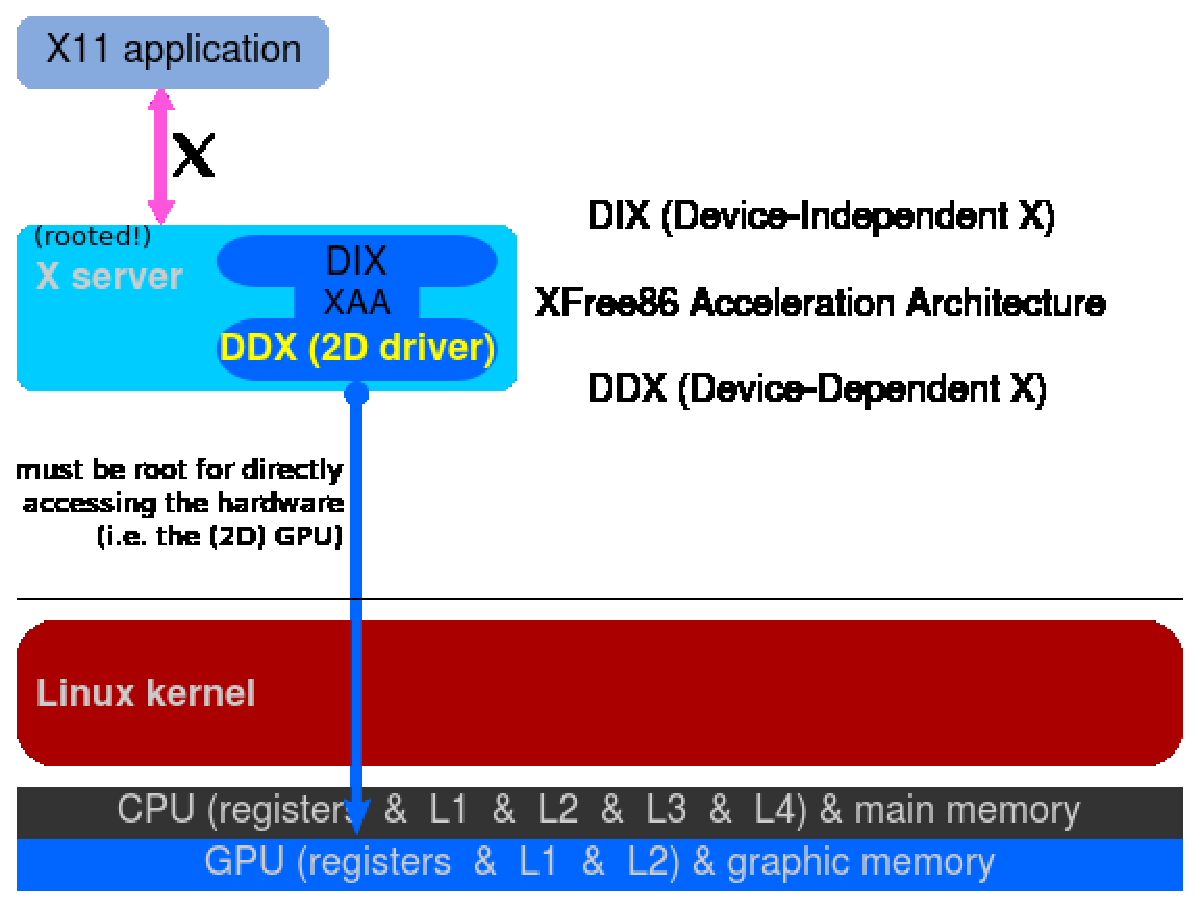
\includegraphics[width=10cm,height=6cm]{figures/chap01/Linux_graphics_drivers_2D}
  \caption{早期Linux下2D图形系统体系栈}
  \label{fig:2D-Graph-Stack}
\end{figure}

\subsubsection{支持3D图形渲染的Linux图形体系栈}
经过不断的发展,Linux通过OpenGL实现了3D图形渲染,其中3D图形渲染的方法主要有两种:
\begin{itemize}
\item{\textbf{Indirect Rendering}}: \\
在一些传统的系统平台上,由于只能唯一通过X-Server访问图形硬件,所以只能向X-Server发送绘制指令然后再通过X-Server转化为硬件命令给GPU执行,这种方式和传统的2D绘制方式相似。
\item{\textbf{Direct Rendering}}: \\ 
随着系统平台上的发展,直接渲染框架(Direct Rendering Infrastructure)的诞生使得OpenGL程序可以通过Linux内核的drm库直接与图形硬件(GPU)进行交互,这一进步极大的提高了3D渲染的效率,成为当今比较主流的渲染方式。
\end{itemize}

\begin{figure}[H] 
  \centering
  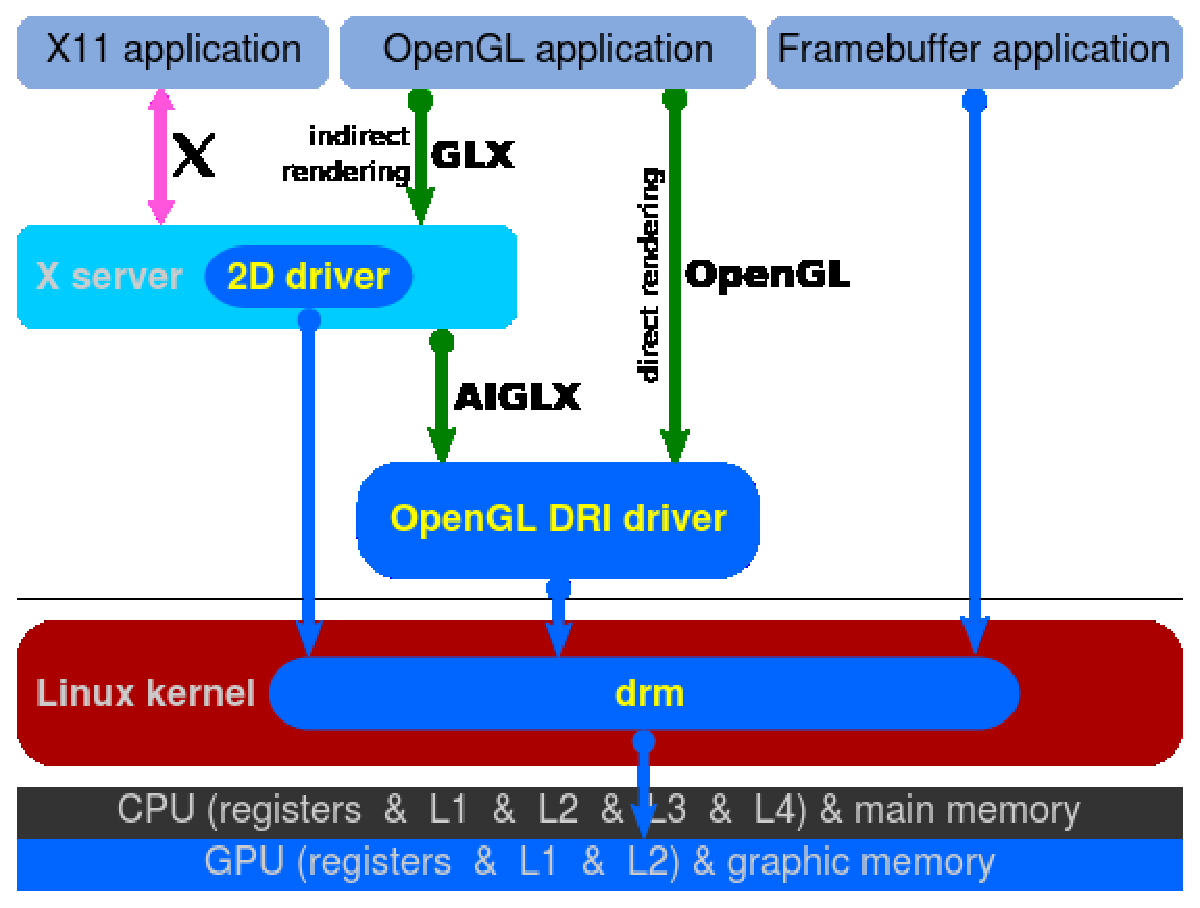
\includegraphics[width=10cm,height=6cm]{figures/chap01/OpenGL_With_Direct_Rendering}
  \caption{Linux下3D图形系统体系栈}
  \label{fig:OpenGL_With_Direct_Rendering}
\end{figure}



\subsection{OpenGL}

\subsubsection{OpenGL基本介绍}
开放图形库(Open Graphics Library,缩写为OpenGL)是个定义了一个跨编程语言、跨平台的应用程序接口(API)的规范,它用于生成2D、3D图像。这个接口由近350个不同的函数调用组成,用来从简单的图形比特绘制复杂的三维景象。而另一种程序接口系统是仅用于Microsoft Windows上的Direct3D。OpenGL常用于CAD、虚拟实境、科学可视化程序和电子游戏开发。

OpenGL规范描述了绘制2D和3D图形的抽象API。尽管这些API可以完全通过软件实现,但它是为大部分或者全部使用硬件加速而设计的。OpenGL不仅语言无关,而且平台无关。规范只字未提获得和管理OpenGL上下文相关的内容,而是将这些作为细节交给底层的窗口系统。出于同样的原因,OpenGL纯粹专注于渲染,而不提供输入、音频以及窗口相关的API。

\subsubsection{OpenGL渲染管线}

绝大多数OpenGL实现都有着相似的操作,一系列相关的处理阶段叫做OpenGL渲染管线。图\ref{fig:OpenGL-Pipeline}显示了这些顺序,几何数据(顶点、直线和多边形)所经历的处理阶段包括求值器和基于顶点的操作,而像素数据(像素、图像和位图)的处理过程则有所不同。在最终的像素数据写入到帧缓存之前,这两种类型的数据都经过相同的最终步骤(光栅化和基于片段的操作)\cite{OpenGL-Programming-Guide}。

\begin{figure}[H] 
  \centering
  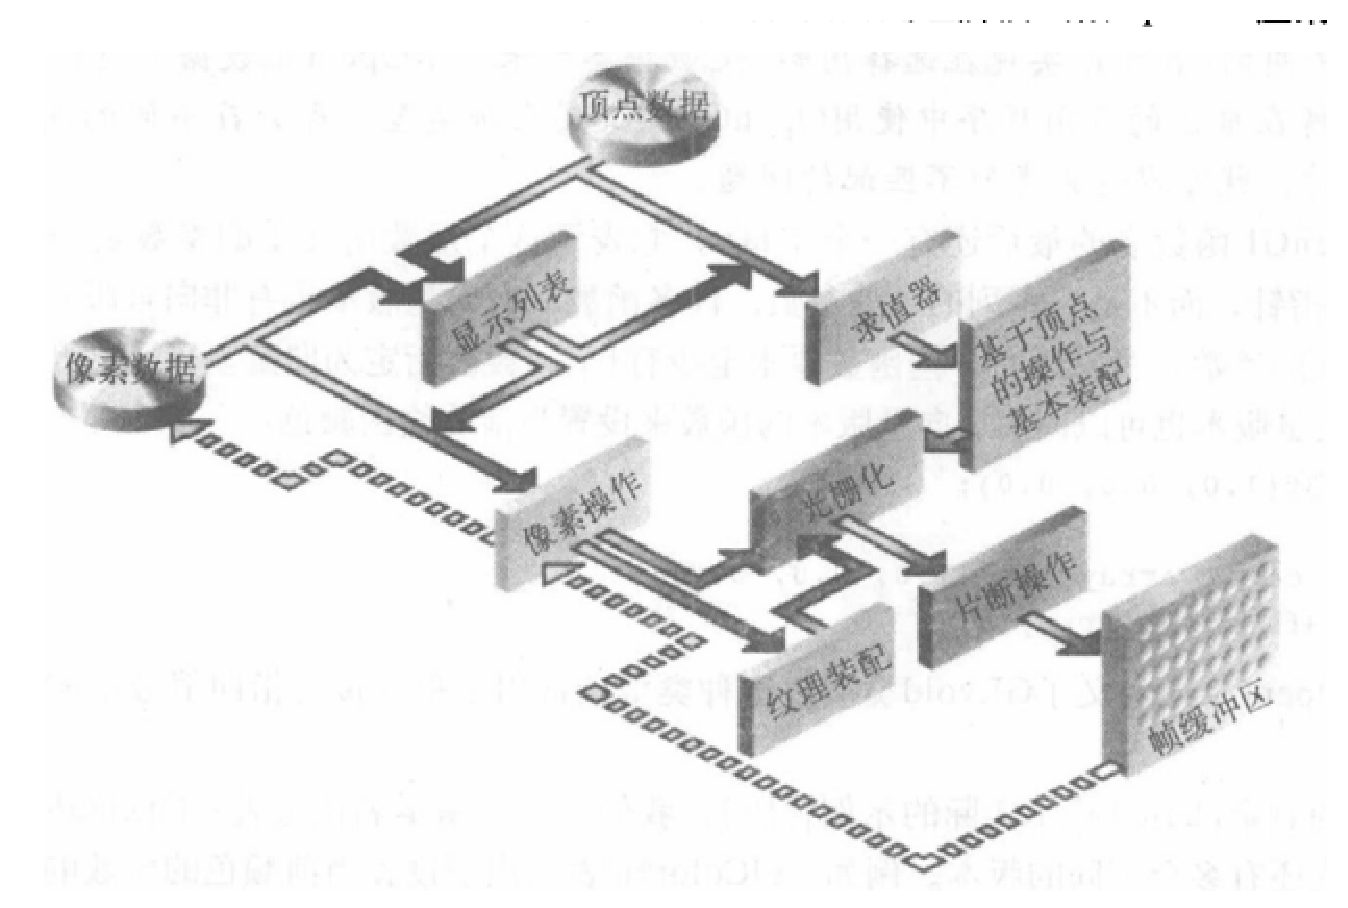
\includegraphics[width=10cm,height=7cm]{figures/chap01/OpenGL-Pipeline}
  \caption{OpenGL渲染管线}
  \label{fig:OpenGL-Pipeline}
\end{figure}

这里详细介绍一下渲染管线上的几个阶段:
\begin{itemize}
\item{\textbf{显示列表}}:\quad几何图形和像素都可以保存到显示列表中,以供当前或者以后使用。当一个显示列表被执行时候,保存的数据就从显示列表取出,就像在立即模式下直接由应用程序发送的那样。
\item{\textbf{求值器}}:\quad所有的几何图形都最终要通过顶点来表示。求值器提供了一种方法,它根据曲线或者表面的控制顶点计算表示曲线或者表面的顶点。这种方法是一种多项式映射,它可以根据控制点产生表面法线,纹理坐标等。
\item{\textbf{基于顶点的操作与图元装配}}:\quad这其实是两个过程,首先基于顶点的操作是把顶点转化为图元,即将空间坐标从3D世界的一个位置投影到屏幕的一个位置。其次图元装配阶段主要内容就是裁剪,它的任务是消除位于某个特定平面以外的部分几何图元。
\item{\textbf{像素操作}}:\quad通常需要对来自系统内存的一个数组中的像素进行解包,接着这些像素数据会被执行像素转化(缩放、偏移、映射和截取)操作。
\item{\textbf{纹理装配}}:\quad OpenGL应用程序可以在几何物体上应用纹理图像,此阶段就是纹理相关的装配处理。
\item{\textbf{光栅化}}:\quad把几何数据和像素数据转化为片段的过程。每个片段对应于帧缓存的一个像素。这个过程会考虑直线的宽度,点的大小,着色模型以及抗锯齿等计算。
\item{\textbf{片段操作}}:\quad数据实际存储到帧缓存区前,还需要执行的一系列操作,比如可能的纹理操作,前面纹理装配阶段产生的纹理内存会为每个片段生成一个纹理单元并与该片段融合。
\end{itemize}

\subsubsection{OpenGL版本变化}
OpenGL是一个不断进化的API。新版OpenGL规范会定期由Khronos Group发布,新版本通过扩展API来支持各种新功能。每个版本的细节由Khronos Group的成员一致决定,包括显卡厂商、操作系统设计人员以及类似Mozilla和谷歌的一般性技术公司。详细历史版本更新参阅附录\ref{cha:OpenGL-History-Version}。



\section{Mesa3D介绍}

\subsection{Mesa3D简介}
Mesa3D最早是由Brian Paul在1993年8月开始开发的一个实现了OpenGL API的开源图形库\cite{Mesa-Wiki}。它目前隶属于freedesktop.org,广泛运用在Liunx, BSD等操作系统。早期的Mesa3D的图形渲染实现是采用纯软件计算实现的,后来随着图形硬件的飞速发展,Mesa3D则转为使用图形硬件进行加速渲染,它广泛支持目前主流的各种图形硬件设备:
\begin{itemize}
\item{}Intel i965,i945,i915
\item{}AMD Radeon series(r200,r300,r600 etc)
\item{}NVIDIA GPUs
\end{itemize}
Mesa3D不仅支持基本的OpenGL API,而还支持OpenGL ES、OpenVG、OpenCL、VDPAU和EGL等。

\begin{figure}[H] 
  \centering
  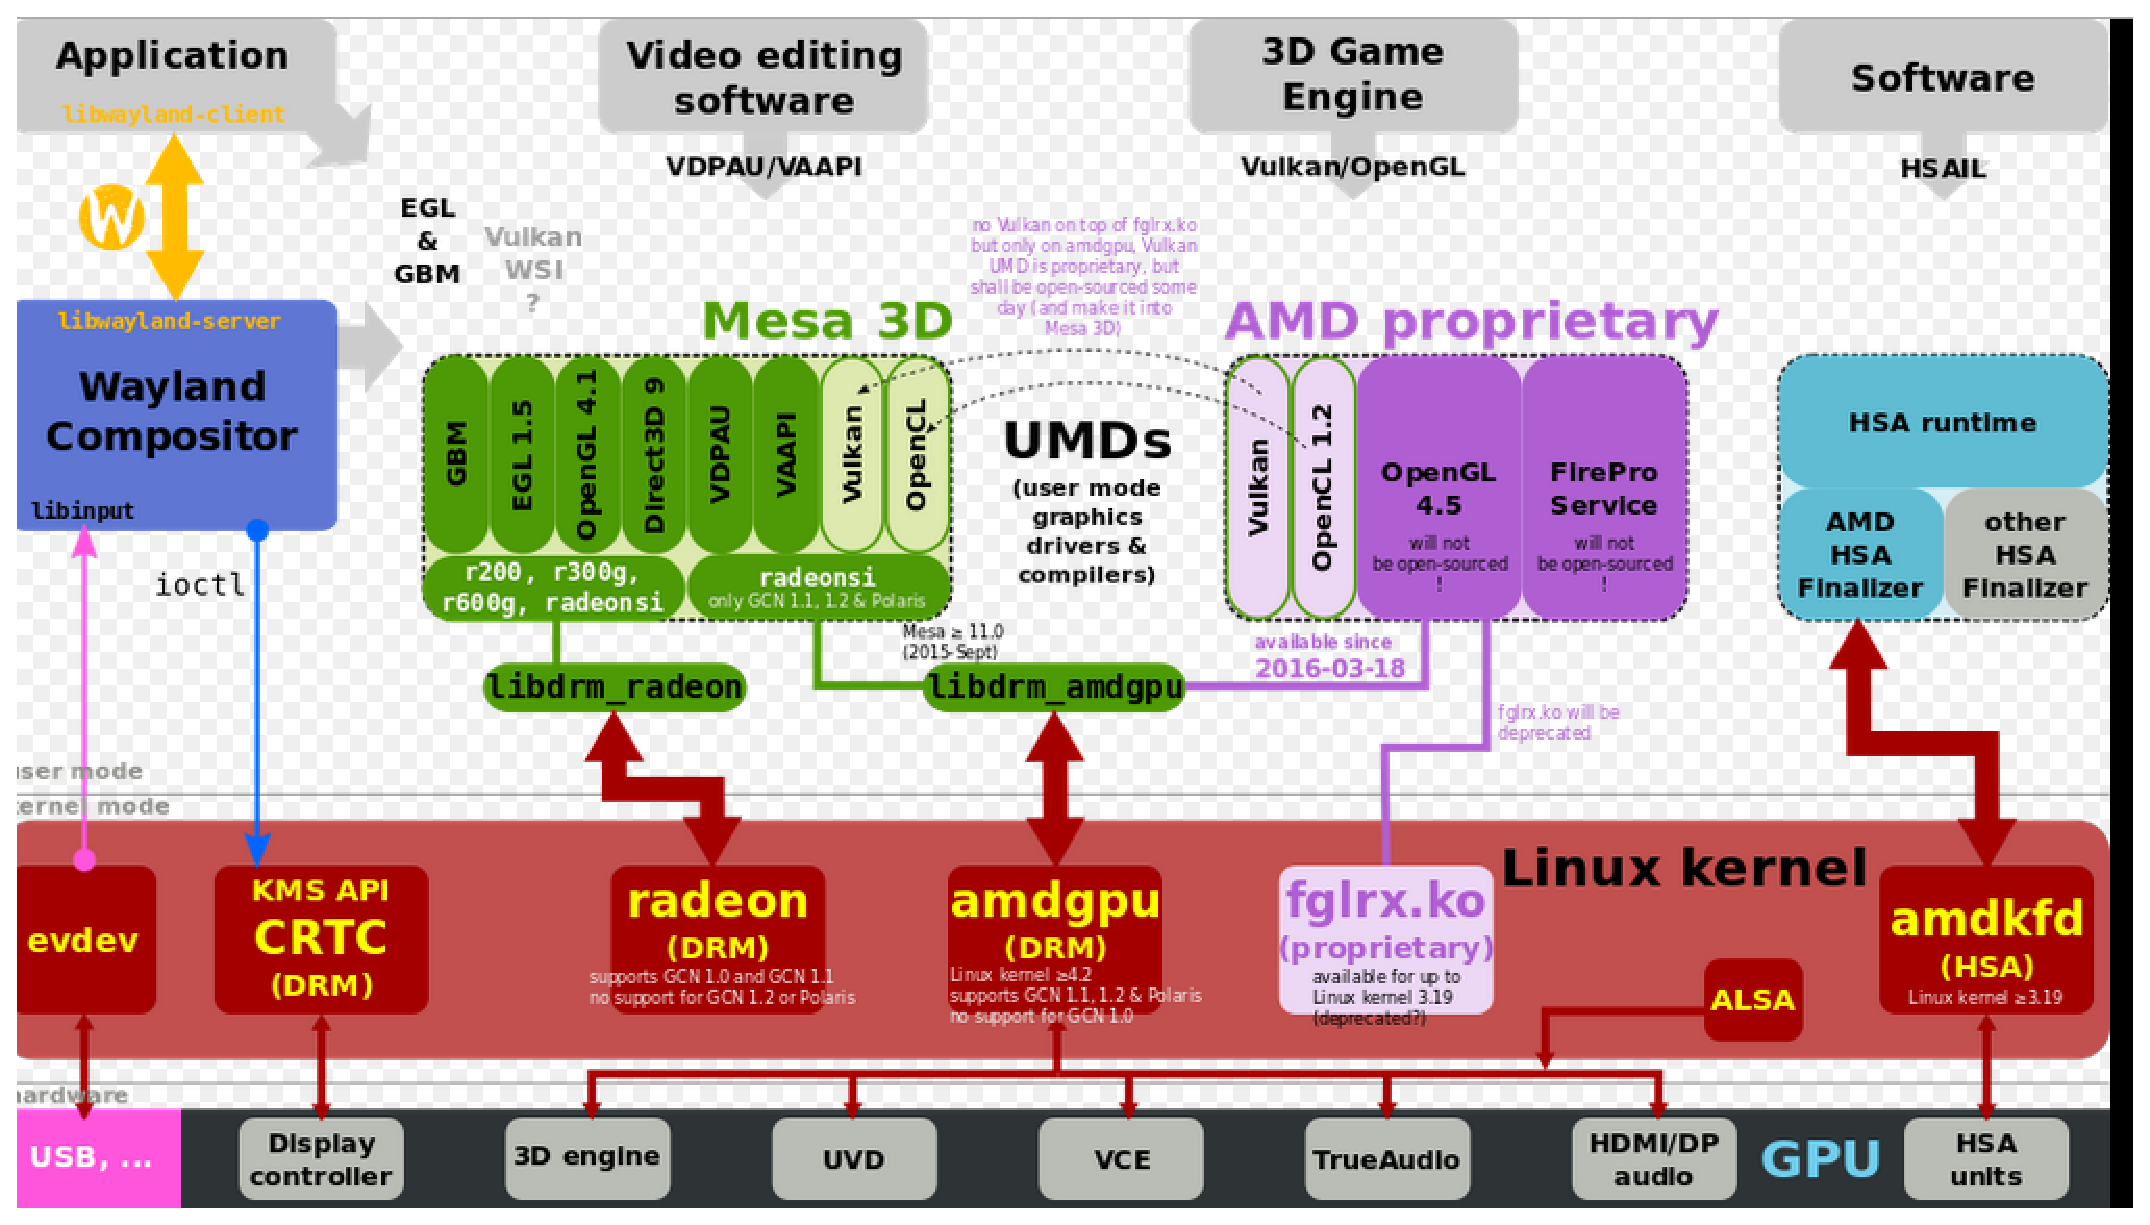
\includegraphics[width=14cm,height=9cm]{figures/chap01/linux-mesa}
  \caption{现代Linux图形栈与Mesa3D}
  \label{fig:linux-mesa}
\end{figure}

\subsection{Mesa3D版本信息}
为了匹配OpenGL的版本不断变化以及各大图形硬件厂商的图形设备不断更新,Mesa3D也一直不断的更新新的版本。到目前为止最新的Mesa3D版本为2016年3月更新的Version 11.2,详细版本更新信息以及支持的OpenGL版本见附录\ref{cha:Mesa3D-History-Version}


\section{龙芯系列处理器介绍}


龙芯处理器主要包括三个系列。龙芯1号处理器及其IP系列主要面向嵌入式应用,龙芯2号超标量处理器及其IP系列主要面向桌面应用,龙芯3号多核处理器系列主要面向服务器和高性能机应用。根据应用的需要,其中部分龙芯2号也可以面向部分高端嵌入式应用,部分低端龙芯3号也可以面向部分桌面应用。以后上述三个系列将并行地发展。

龙芯系列处理器通过充分开发指令级并行性、数据级并行性、线程级并行性来提高性能。其中龙芯1号系列微处理器实现了带有静态分支预测和阻塞Cache的单发射乱序执行流水线;龙芯2号系列微处理器实现了带有动态分支预测和非阻塞Cache的超标量四发射乱序执行流水线,以及还使用浮点数据通路复用技术实现了定点的单指令流多数据流指令;龙芯3号基于可伸缩的多核互连架构设计,在单个芯片上集成多个高性能处理器核以及大量的2级Cache,还通过高速I/O接口实现多芯片的互连以组成更大规模的系统。


\section{本文主要贡献}

本文的主要工作内容如下:

\begin{itemize}
\item{\textbf{立即模式(Immediate Mode)\footnote{OpenGL传统的使用glBegin...glEnd方式制定绘制方式,在这两个函数对之间给出绘制的数据,这种方式称为立即模式。}下顶点数据传输过程研究与优化}}: \\
OpenGL的立即模式下,glBegin与glEnd之间的数据会逐次拷贝到顶点缓冲区中,每当顶点缓存去装载满数据后,这些数据会被传输到图形硬件设备(GPU)显存中,然后再继续装载未装载的数据。本文通过分析这个装载过程的性能瓶颈,提出了一种
\item{\textbf{显示列表(Display List)\footnote{OpenGL显示列表是由一组预先存储起来的留待以后调用的OpenGL函数语句组成的,当调用这张显示列表时就依次执行表中所列出的函数语句。}下CPU与GPU负载平衡的优化}}: \\
通过跟踪分析Mesa3D库代码发现在创建显示列表时候,会先预分配一块缓冲区,当数据溢出时会继续分配一块相同大小的缓冲区,重复此过程直到所有数据都存放到缓冲区中然后提交到显存设备中。这样在面临显示列表中包含大量顶点数据时,就需要分配很多次缓存区,这其中涉及到的数据准备和状态管理等操作都需要GPU来做,这便会导致CPU与GPU的工作负载不平衡,形成性能瓶颈。本文通过根据显示列表数据规模确定缓存区大小的优化方法来解决显示列表的性能瓶颈。
\item{\textbf{内存向显存数据传输优化}}: \\
由于Mesa3D中的顶点数据,属性数据等等都需要传输到显存中,所以内存到显存的数据传输效率就显得至关重要。本文研究分析了现有Mesa3D库内存到显存的数据传输过程,提出了一种简化的数据传输拷贝方式,提高了数据传输速度。
\end{itemize}



本文的研究工作均在龙芯3A系列软硬件平台上使用主流OpenGL性能测试集svPerfGL\footnote{svPerfGL是一个开源的OpenGL基准测试集合,它主要用来测量科学可视化应用的真实性能。}进行了测试和验证,其中立即模式性能提升约有xxx,显示列表性能提升约有xxx,内存向显存数据传输优化性能提升约有xxx。本文相关优化成果都已集成到应用到龙芯最新Mesa3D图形库中。


\section{本文组织结构}

本文总共分为六章。

第一章首先介绍了Linux环境下主要图形系统结构、OpenGL和mesa3D的历史与现状,然后介绍了龙芯3A系列处理器的相关技术背景,最后交待了本文的主要工作和组织结构。

第二章主要介绍Mesa3D的主要结构和工作原理。重点对Mesa3D渲染管线实现原理和缓存区管理策略进行研究和分析,并对Mesa3D国内外相关的优化现状与优化成果进行总结。

第三章主要介绍Mesa3D缓存策略的优化。包括两方面的内容:第一是关于立即模式下数据缓存策略的原理分析,并结合龙芯3A实际平台特点进行优化;第二是关于显示列表模式下,数据缓存策略的原理分析,同样根据龙芯3A实际平台特点进行优化。

第四章主要介绍Mesa3D中的内存到显存数据传输的优化。研究和分析了原有Mesa3D中数据从内存传输到显存的传输链路,结合龙芯3A平台数据拷贝性能特点,提出了一个简化而又高效的数据传输链路,从而提高内存到显存的数据传输效率。

第五章主要是优化结果性能测试与分析部分。采用svPerfGL测试基准对前面提出的各个优化方法进行测试提升效果,并对结果进行分析。

第六章主要是对全文研究工作进行总结,并针对研究中遇到的一些问题,提出未来研究的方向。



%%% Local Variables: 
%%% mode: latex
%%% TeX-master: t
%%% End: 

\chapter{中华人民共和国}
\label{cha:china}

\section{其它例子}
\label{sec:other}

在第\chapterref{cha:intro}章中我们学习了贝叶斯公式~(\ref{equ:chap1:bayes}),这里我们复
习一下:
\begin{equation}
\label{equ:chap2:bayes}
p(y|\mathbf{x}) = \frac{p(\mathbf{x},y)}{p(\mathbf{x})}=
\frac{p(\mathbf{x}|y)p(y)}{p(\mathbf{x})} 
\end{equation}

\subsection{绘图}
\label{sec:draw}

本模板不再预先装载任何绘图包(如 \textsf{pstricks,pgf} 等),完全由你自己来决定。
个人觉得 \textsf{pgf} 不错,不依赖于 Postscript。此外还有很多针对 \LaTeX{} 的
 GUI 作图工具,如 XFig(jFig), WinFig, Tpx, Ipe, Dia, Inkscape, LaTeXPiX,
jPicEdt, jaxdraw 等等。

\subsection{插图}
\label{sec:graphs}

强烈推荐《\LaTeXe 插图指南》!关于子图形的使用细节请参看 \textsf{subcaption} 宏包的说明文档。

\subsubsection{一个图形}
\label{sec:onefig}
一般图形都是处在浮动环境中。之所以称为浮动是指最终排版效果图形的位置不一定与源文
件中的位置对应\footnote{This is not a bug, but a feature of \LaTeX!},这也是刚使
用 \LaTeX{} 同学可能遇到的问题。如果要强制固定浮动图形的位置,请使用 \textsf{float} 宏包,
它提供了 \texttt{[H]} 参数,比如图~\ref{fig:xfig1}。
\begin{figure}[H] % use float package if you want it here
  \centering
  \includegraphics{hello}
  \caption{利用 Xfig 制图}
  \label{fig:xfig1}
\end{figure}

大学之道,在明明德,在亲民,在止于至善。知止而后有定;定而后能静;静而后能安;安
而后能虑;虑而后能得。物有本末,事有终始。知所先后,则近道矣。古之欲明明德于天
下者,先治其国;欲治其国者,先齐其家;欲齐其家者,先修其身;欲修其身者,先正其心;
欲正其心者,先诚其意;欲诚其意者,先致其知;致知在格物。物格而后知至;知至而后
意诚;意诚而后心正;心正而后身 修;身修而后家齐;家齐而后国治;国治而后天下
平。自天子以至于庶人,壹是皆以修身为本。其本乱而未治者 否矣。其所厚者薄,而其所
薄者厚,未之有也!

\hfill ——《大学》


\subsubsection{多个图形}
\label{sec:multifig}

如果多个图形相互独立,并不共用一个图形计数器,那么用 \verb|minipage| 或者
\verb|parbox| 就可以。否则,请参看图~\ref{fig:big1-subcaptionbox},它包含两个小图,分别是图~\ref{fig:subfig1} 
和图~\ref{fig:subfig2}。推荐使用\verb|\subcaptionbox|,
因为可以像图~\ref{fig:big1-subcaptionbox} 那样对齐子图的标题,
也可以使用\textsf{subcaption}宏包的\verb|\subcaption|(放在minipage中,用法同\verb|\caption|)
或是 subfigure 、 subtable环境,像图~\ref{fig:big1-subfigure},不要再用 \verb|\subfloat|、
\verb|\subfigure| 和 \verb|\subtable|。
\begin{figure}[h]
  \centering%
  \subcaptionbox{第一个小图形\label{fig:subfig1}}
  [3cm] %标题的长度,超过则会换行,如下一个小图。
    {
\includegraphics[height=3cm]{thu-fig-logo}}
      \hspace{4em}%
  \subcaptionbox{第二个小图形,注意这个图略矮些。如果标题很长的话,它会自动换行\label{fig:subfig2}}
      {
\includegraphics[height=2cm]{thu-text-logo}}
  \caption{包含子图形的大图形(subcaptionbox示例)}
  \label{fig:big1-subcaptionbox}
\end{figure}
\begin{figure}[h]
  \centering%
  \begin{subfigure}{3cm}
    
\includegraphics[height=3cm]{thu-fig-logo}
    \caption{第一个小图形}
  \end{subfigure}
  \hspace{4em}%
  \begin{subfigure}{0.5\textwidth}
    
\includegraphics[height=2cm]{thu-text-logo}
    \caption{第二个小图形,注意这个图略矮些。subfigure中同一行的子图在顶端对齐。}
  \end{subfigure}
  \caption{包含子图形的大图形(subfigure示例)}
  \label{fig:big1-subfigure}
\end{figure}
古之学者必有师。师者,所以传道受业解惑也。人非生而知之者,孰能无惑?惑而不从师,
其为惑也,终不解矣。生乎吾前,其闻道也固先乎吾,吾从而师之;生乎吾後,其闻道也亦
先乎吾,吾从而师之。吾师道也,夫庸知其年之先後生於吾乎!是故无贵无贱无长无少,道
之所存,师之所存也。

嗟乎!师道之不传也久矣,欲人之无惑也难矣。古之圣人,其出人也远矣,犹且从师而问焉;
今之众人,其下圣人也亦远矣,而耻学於师。是故圣益圣,愚益愚。圣人之所以为圣,愚
人之所以为愚,其皆出於此乎?爱其子,择师而教之,於其身也,则耻师焉,惑焉。彼童子
之师,授之书而习其句读者,非吾所谓传其道、解其惑者也。句读之不知,惑之不解,或师
焉,或不焉,小学而大遗,吾未见其明也。巫医、乐师、百工之人不耻相师,  士大夫之族
曰“师”曰“弟子”之云者,则群聚而笑之。问之,则曰:彼与彼年相若也,道相似也,位
卑则足羞,官盛则近谀。呜呼!师道之不复,可知矣。巫医、乐师、百工之人。吾子不齿,
今其智乃反不能及,其可怪也欤!圣人无常师。孔子师郯子、苌子、师襄、老聃。郯子之徒,
其贤不及孔子。孔子曰:“三人行,必有我师。”是故弟子不必不如师,师不必贤於弟子。
闻道有先後,术业有专攻,如是而已。

如果要把编号的两个图形并排,那么小页就非常有用了:
\begin{figure}
\begin{minipage}{0.48\textwidth}
  \centering
  
\includegraphics[height=2cm]{thu-whole-logo}
  \caption{并排第一个图}
  \label{fig:parallel1}
\end{minipage}\hfill
\begin{minipage}{0.48\textwidth}
  \centering
  
\includegraphics[height=2cm]{thu-whole-logo}
  \caption{并排第二个图}
  \label{fig:parallel2}
\end{minipage}
\end{figure}

李氏子蟠,年十七,好古文、六艺,经传皆通习之,不拘於时,学於余。余嘉其能行古
道,作师说以贻之。

\hfill —— 韩愈(唐)



\chapter{Mesa3D的性能优化技术}

\section{Mesa3D的CPU与GPU负载平衡的优化}

\subsection{研究背景}

\subsection{Mesa3D图形库CPU与GPU负载关系}

\subsection{系统设计}

\section{Mesa3D的内存到显存的数据传输的优化}

\subsection{研究背景}

\subsection{原有内存到显存的数据传输方式}

\subsection{内存到显存的数据传输方式的改进方式}

\section{Mesa3D的CPU端计算优化}

\subsection{研究背景}

\subsection{CPU端计算热点}

\subsection{CPU端优化技术}

\section{本章小结}


\chapter{测试与验证}

\section{测试与验证平台介绍}

\section{CPU与GPU负载平衡优化测试}

\section{内存与显存数据传输优化测试}

\section{本章小结}


\chapter{总结与展望}

\section{本文工作总结}

\section{未来研究方向}


% 参考文献
\bibliographystyle{GBT7714-2005NLang-UTF8}
\bibliography{ref/refs}

% 附录
\begin{appendix}
%%% Local Variables: 
%%% mode: latex
%%% TeX-master: "../main"
%%% End: 

\chapter{OpenGL历史版本变更表 }
%\footnote{摘自OpenGL-维基百科}
\label{cha:OpenGL-History-Version}

%跨页表格
\begin{center} \tablecaption{OpenGL版本变更表 \label{tab:OpenGL-Version-History}} 
\tablefirsthead{
\rowcolor[gray]{0.8}
\multicolumn{1}{l}{\textbf{主要版本}} &
\multicolumn{1}{l}{\textbf{发布日期}} &
\multicolumn{1}{c}{\textbf{重要变更}} \\ }
\tablehead{\multicolumn{3}{c}{
\small 表 \ref{tab:OpenGL-Version-History} (续) } \\
\rowcolor[gray]{0.8}
\multicolumn{1}{l}{\textbf{主要版本}} &
\multicolumn{1}{l}{\textbf{发布日期}} &
\multicolumn{1}{c}{\textbf{重要变更}} \\ }
\tabletail{\bottomrule
\multicolumn{3}{c}{\small 接下页} \\}
\tablelasttail{\bottomrule}

\begin{supertabular}{p{2.cm}p{2.cm}p{11.cm}}
      1.1 & 1997.1 & \\
      1.2 & 1998.3 & \\
      1.2.1 & 1998.10 & \\
      1.3 & 2001.8 & \\
      1.4 & 2002.7 & \\
      1.5 & 2003.7 & \\
      2.0 & 2004.9 & \\
      2.1 & 2006.7 & \\
      3.0 & 2008.8 & \\
      3.1 & 2009.3 & \\
      3.2 & 2009.8 & \\
      3.3 & 2010.3 & \\
      4.0 & 2010.3 & \\
      4.1 & 2010.7 & \\
      4.2 & 2011.8 & 
支持的显卡: \\
& & Nvidia GeForce 400 series, Nvidia GeForce 500 series, Nvidia GeForce 600 series, ATI Radeon HD 5000 series, AMD Radeon HD 6000 Series, AMD Radeon HD 7000 Series \\
& & \tabitem 支持Shaders原子计数器和加载、存储、原子读-修改-写操作的单级纹理着色器。\\
& & \tabitem捕捉GPU-tessellated几何变换反馈的结果绘制的多个实例,使复杂的对象进行有效的重新定位和复制。\\
& & \tabitem支持修改任意子集的压缩纹理,而无需重新下载整个GPU的纹理,显著的性能改进。\\
& & \tabitem支持包装成一个单一的32位值显著降低内存存储和带宽的高效着色处理多个8位和16位值。\\
    %\toprule[1.5pt] 
      4.3 & 2012.8 & 支持的显卡: \\
& & NVIDIA GeForce400系列,NVIDIA GeForce500系列,NVIDIA GeForce600系列,NVIDIA GeForce700系列,ATI Radeon HD 5000系列,AMD Radeon HD6000系列,AMD Radeon HD7000系列,AMD Radeon HD8000系列 \\
& & \tabitem 围内充分利用GPU的并发计算着色器的图形管道 \\
& & \tabitem 暗器的存储缓冲器对象 \\
& & \tabitem 纹理参数查询 \\
& & \tabitem 作为标准功能的高质量的纹理压缩ETC2/EAC \\
& & \tabitem 完全兼容的OpenGL ES3.0的API \\
& & \tabitem 在应用程序开发过程中调试能力接收调试消息 \\
& & \tabitem 没有数据复制以不同的方式解释纹理的纹理意见 \\
& & \tabitem 增加了内存的安全性 \\
& & \tabitem 一个多应用的健壮性扩展 \\
      4.4 & 2013.7 & 支持的显卡: \\
& & DIA GeForce 400系列、NVIDIA GeForce 500系列、NVIDIA GeForce 600系列、NVIDIA GeForce 700系列,ATI Radeon HD 5000系列、AMD Radeon HD6000系列、AMD Radeon HD7000系列、AMD Radeon R9/R7 200系列 \\
& & \tabitem 缓冲器位置控制 \\
& & \tabitem 高效异步查询 \\
& & \tabitem 着色器可变布局 \\
& & \tabitem 高效多对象绑定 \\
& & \tabitem 精简化Direct3D应用的移植 \\
& & \tabitem 非绑定的纹理扩展 \\
& & \tabitem 稀疏纹理扩展 \\
      4.5 & 2014.8 & \\
\end{supertabular}
\end{center}

\chapter{Mesa3D历史版本变更表}
\label{cha:Mesa3D-History-Version}

\begin{center} \tablecaption{Mesa3D版本变更表(4.0之前版本不再支持) \label{tab:Mesa3D-Version-History}} 
\tablefirsthead{
\rowcolor[gray]{0.8}
\multicolumn{1}{l}{\textbf{主要版本}} &
\multicolumn{1}{l}{\textbf{发布日期}} &
\multicolumn{1}{c}{\textbf{支持OpenGL版本}} \\ }
\tablehead{\multicolumn{3}{c}{
\small 表 \ref{tab:OpenGL-Version-History} (续) } \\
\rowcolor[gray]{0.8}
\multicolumn{1}{l}{\textbf{主要版本}} &
\multicolumn{1}{l}{\textbf{发布日期}} &
\multicolumn{1}{c}{\textbf{支持OpenGL版本}} \\ }
\tabletail{\bottomrule
\multicolumn{3}{c}{\small 接下页} \\}
\tablelasttail{\bottomrule}

\begin{supertabular}{p{2.cm}p{2.cm}m{11.cm}}
      11.2 & 2016.3 & 4.2(Intel 3.3)\\
      11.1 & 2015.12 & 4.2(Intel 3.3)\\
      11.0 & 2015.9 & 4.2(Intel 3.3)\\
      10.6 & 2015.6 & 3.3\\
      10.5 & 2015.3 & 3.3\\
      10.4 & 2014.12 & 3.3\\
      10.3 & 2014.9 & 3.3\\
      10.2 & 2014.6 & 3.3\\
      10.1 & 2014.3 & 3.3\\
      10.0 & 2013.11 & 3.3\\
      9.0 & 2012.10 & 3.1\\
      8.0 & 2012.2 & 3.0\\
      7.0 & 2007.6 & 2.1\\
      6.0 & 2004.1 & 1.5\\
      5.0 & 2002.11 & 1.4\\
      4.0 & 2001.10 & 1.3\\
\end{supertabular}
\end{center}


\chapter{ATTR宏函数}
%\footnote{摘自OpenGL-维基百科}
\label{cha:attr}

\begin{lstlisting}
/**
 * This macro is used to implement all the glVertex, glColor, glTexCoord,
 * glVertexAttrib, etc functions.
 */
#define ATTR( A, N, T, V0, V1, V2, V3 )					\
do {									\
   struct vbo_exec_context *exec = &vbo_context(ctx)->exec;		\
									\
   if (unlikely(!(ctx->Driver.NeedFlush & FLUSH_UPDATE_CURRENT)))	\
      ctx->Driver.BeginVertices( ctx );					\
   									\
   if (unlikely(exec->vtx.active_sz[A] != N))				\
      vbo_exec_fixup_vertex(ctx, A, N);					\
   									\
   {									\
      GLfloat *dest = exec->vtx.attrptr[A];				\
      if (N>0) dest[0] = V0;						\
      if (N>1) dest[1] = V1;						\
      if (N>2) dest[2] = V2;						\
      if (N>3) dest[3] = V3;						\
      exec->vtx.attrtype[A] = T;                                        \
   }									\
									\
   if ((A) == 0) {							\
      /* This is a glVertex call */					\
      GLuint i;								\
									\
      for (i = 0; i < exec->vtx.vertex_size; i++)			\
	 exec->vtx.buffer_ptr[i] = exec->vtx.vertex[i];			\
									\
      exec->vtx.buffer_ptr += exec->vtx.vertex_size;			\    
									\
      /* Set FLUSH_STORED_VERTICES to indicate that there's now */	\
      /* something to draw (not just updating a color or texcoord).*/	\
      ctx->Driver.NeedFlush |= FLUSH_STORED_VERTICES;			\
									\
      if (++exec->vtx.vert_count >= exec->vtx.max_vert)			\
	 vbo_exec_vtx_wrap( exec );					\
   }									\
} while (0)
\end{lstlisting}



\end{appendix}

%%% 其他部分
\backmatter

% 致谢
%%% Local Variables:
%%% mode: latex
%%% TeX-master: "../main"
%%% End:

\begin{ack}
值此论文完成之际,谨向多年来所有关心和帮助过我的人们表达我最诚挚的谢意!

首先要感谢我的导师胡伟武老师,没有他的悉心指导和帮助,本论文的研究工作不可能顺利完成。胡老师严肃的科学态度、严谨的治学精神、精益求精的工作态度和事必躬行的处世作风给我留下非常深刻的印象,必将使我一生受益。在此,谨向尊敬的胡老师致以深深的敬意和衷心的感谢。

其次我还要感谢微处理器研究中心的章隆兵老师、王剑老师、沈海华老师和高翔老师,感谢他们在我的学习、生活和科研过程中都给予了我大量的指导和帮助。此外还要感谢龙芯系统研发部的王洪虎前辈、朱琛师兄、陈建同学、吴博雅同学、李贺斌同学、詹成君同学和宋林枫同学等,感谢他们在我的研究工作中,无私的解答我的一些工程问题,为我的论文研究工作提供了大量的帮助。

还要感谢这篇论文所涉及到的各位学者。本文引用了数位学者的研究文献,他们的大量前期探索为本文研究内容奠定了扎实的基础,使得本文能够在更高的层次上开展工作。

感谢我的父母。你们无私地给予我关心、照顾和支持,与我共同承担这艰苦三年中的喜怒哀乐。家是休憩的港湾,每一次遭受挫折或是获得成就之后,我都能从家里汲取力量再次启航。感谢他们对我永无止境的关爱!

最后,郑重的向我的挚友汪同学表示感谢,感谢你的理解与支持,此生有卿,何其幸哉。

\end{ack}


% 作者简介
\begin{resume}

\noindent
姓名:胡庆海  性别:男  出生日期:1991.10.18  籍贯:安徽\\

\noindent
2013.9 -- 现在      中国科学院计算技术研究所\quad微处理器研究中心\qquad硕士

\noindent
2009.9 -- 2013.7     中国科学技术大学\quad计算机科学与技术系\qquad本科\\

  \resumeitem{攻读硕士学位期间参加的科研项目} % 有就写,没有就删除
  \begin{enumerate}[{[}1{]}]
  \item 龙芯平台QT库优化, 2014年11月~2015年6月
  \item 龙芯平台Mesa库优化, 2015年9月~2016年2月 
  \end{enumerate}

  \resumeitem{攻读硕士学位期间的获奖情况} % 有就写,没有就删除
  \begin{enumerate}[{[}1{]}]
  \item  2015年被评为中国科学院“三好学生”
  \end{enumerate}
\end{resume}


% 保证总页数为偶数。连续双面打印时,防止将两份论文的末页、首页打印在同一张纸上。
\cleardoublepage

\end{document}
